\documentclass[10pt,twocolumn]{article}
\usepackage{xcolor}
\usepackage{comment}
\usepackage{graphicx}
\usepackage{multicol,graphicx}
\usepackage{multirow}
\usepackage{multicol}
\usepackage{subcaption}
\usepackage{tikz}
\usepackage{hyperref}
\usepackage[export]{adjustbox}
\usepackage{circuitikz}
\usepackage{siunitx} %to allign according to decimal point
\usepackage{algorithm2e}
\usepackage{amsmath}
\usepackage{systeme}
\usepackage{lipsum}
\usepackage{blindtext}

\begin{document}
	\title{Preparing Document in LaTex}
	\author{Priyanshu Singh}
	\date{\today}
	\maketitle
	\blindtext
	\begin{figure}[h]
		\centering
		\begin{subfigure}{0.2\textwidth}
			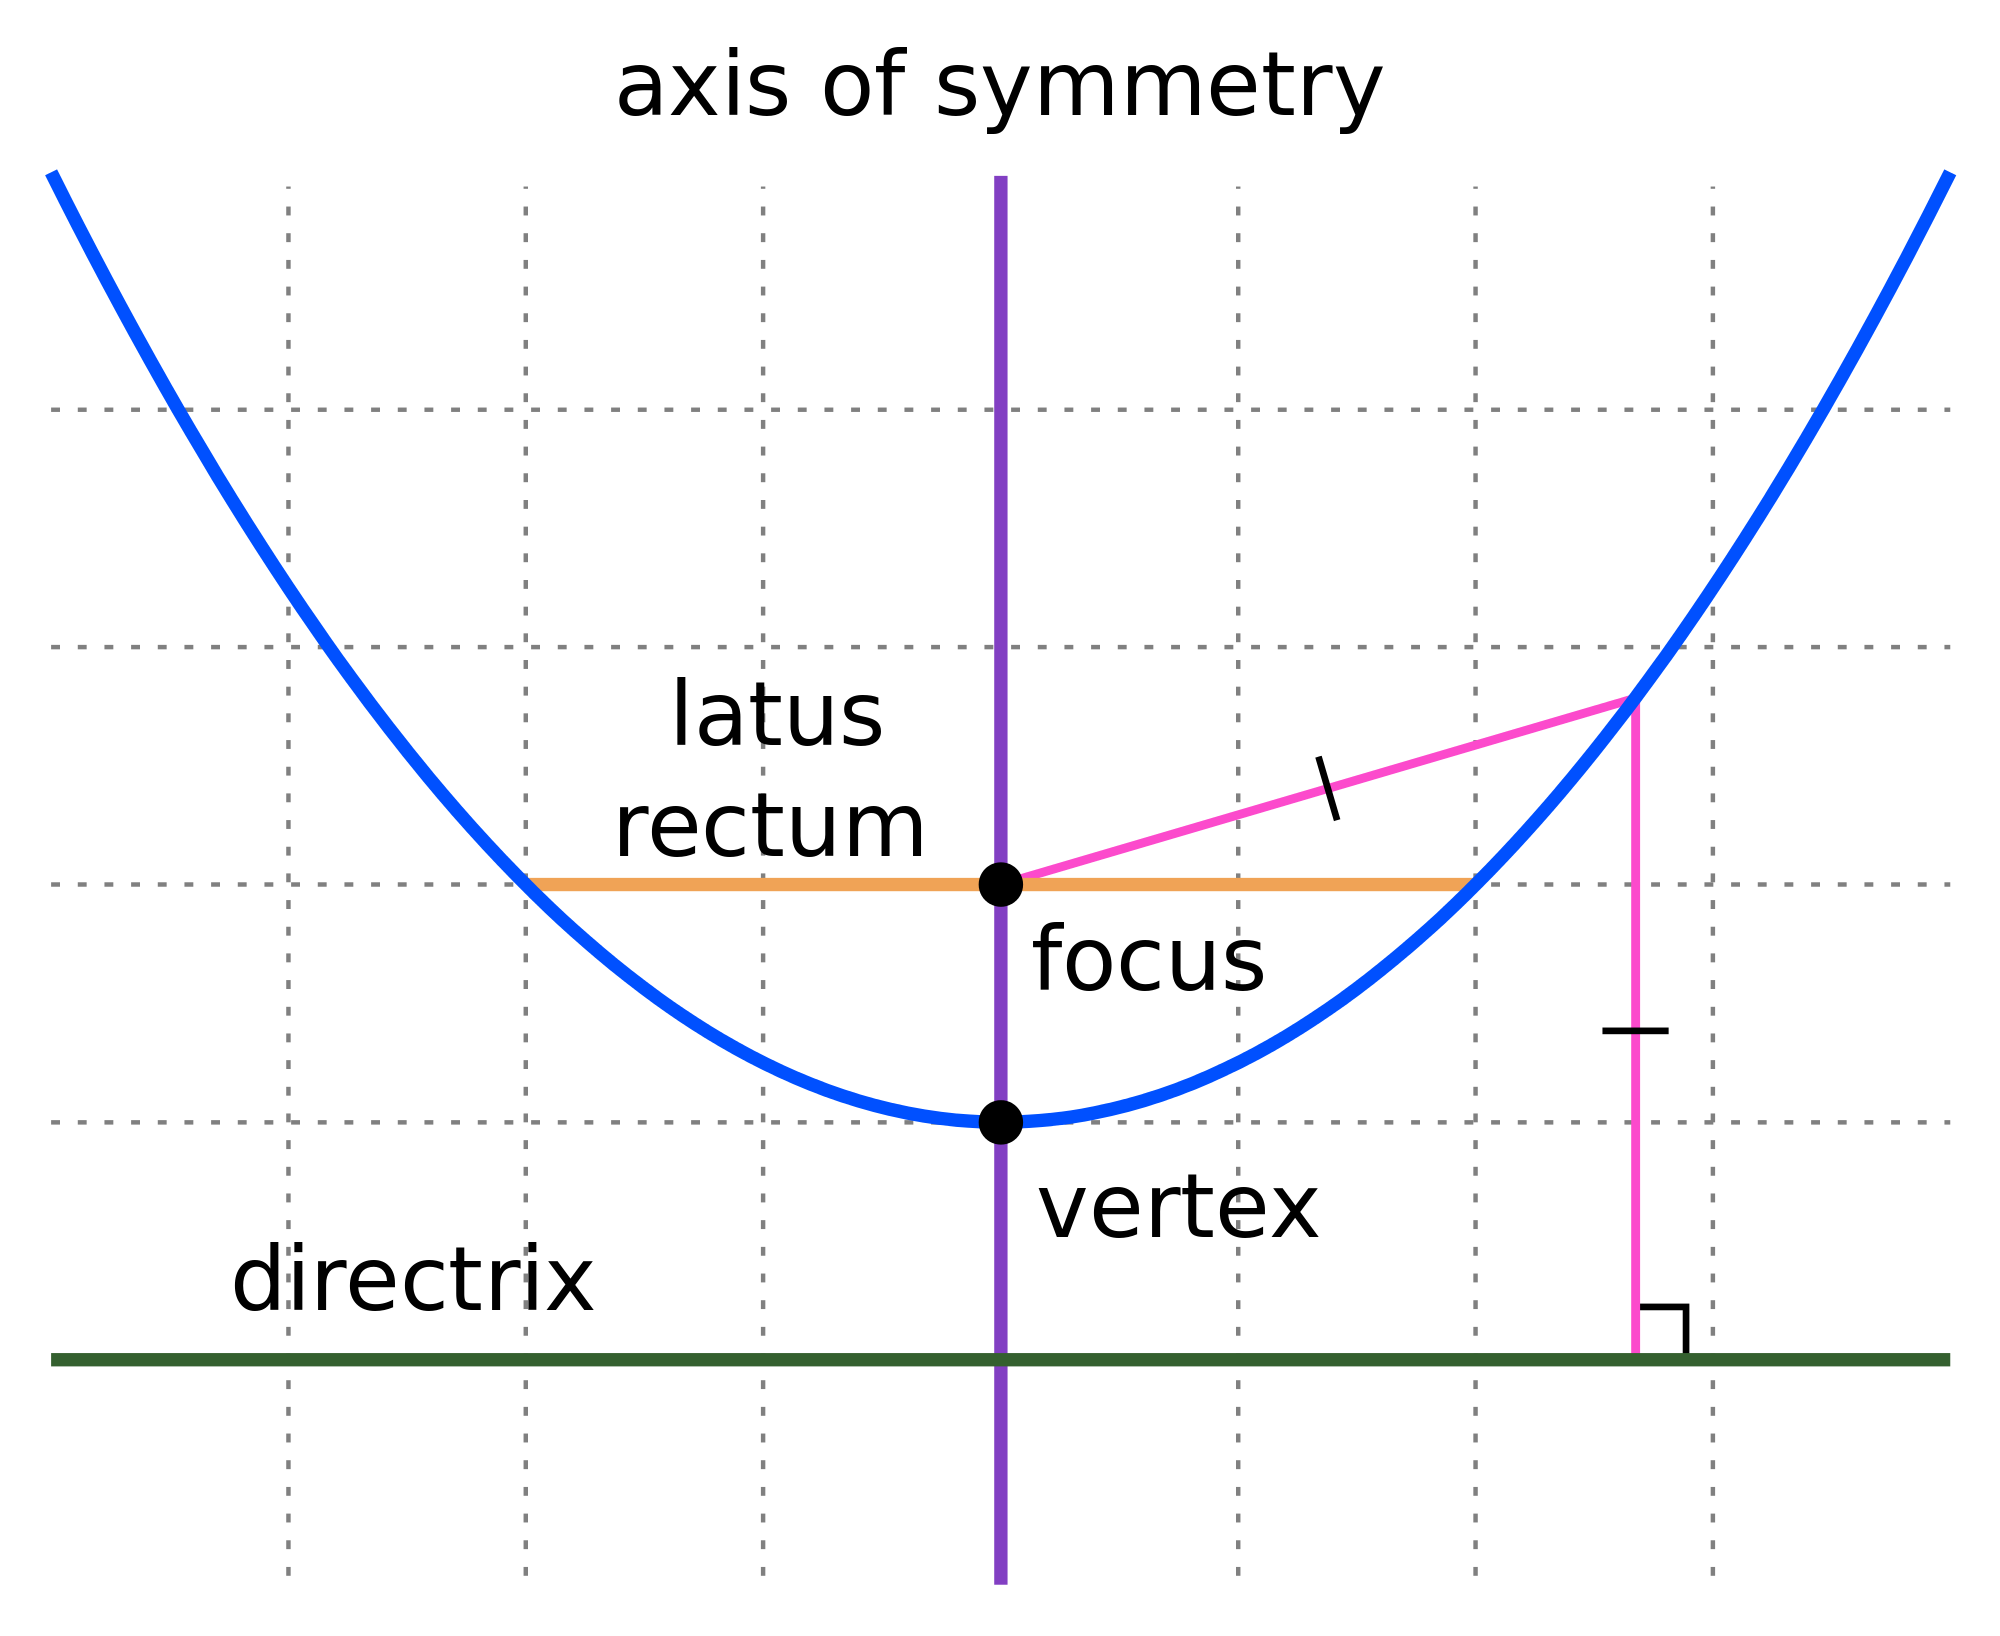
\includegraphics[width=1\textwidth,right]{parabola}
			%\centering
		\end{subfigure}
		\begin{subfigure}{0.2\textwidth}
			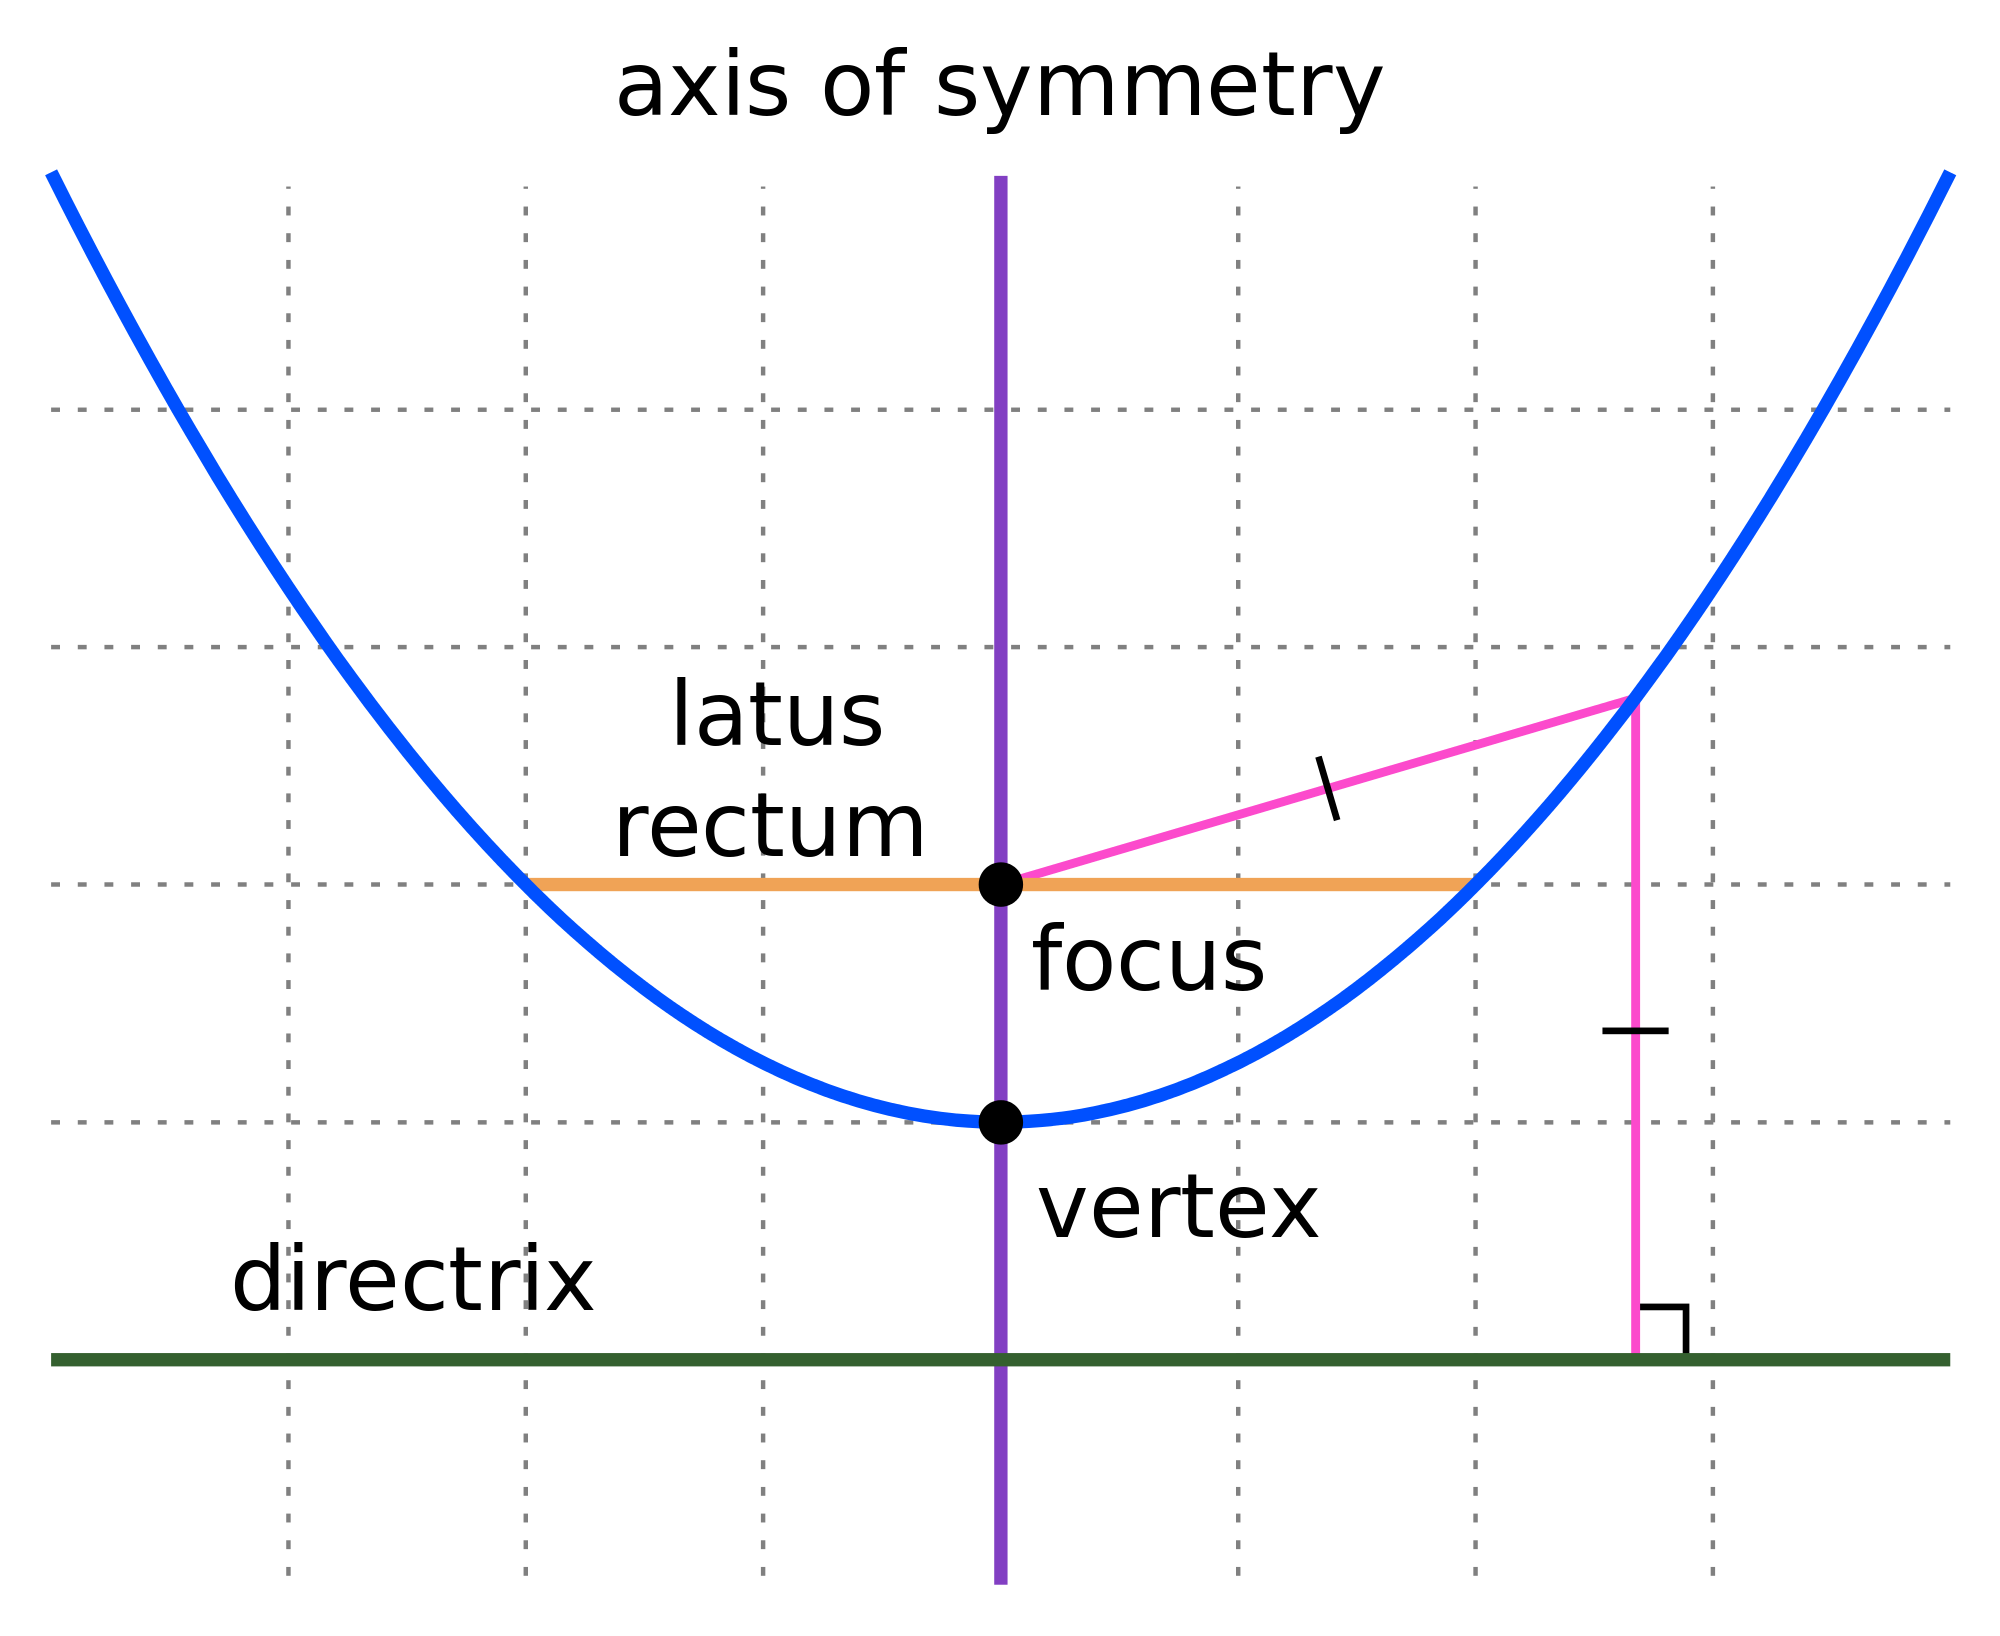
\includegraphics[width=1\textwidth,left]{parabola}
			%\centering
		\end{subfigure}\\
		\begin{subfigure}{0.2\textwidth}
			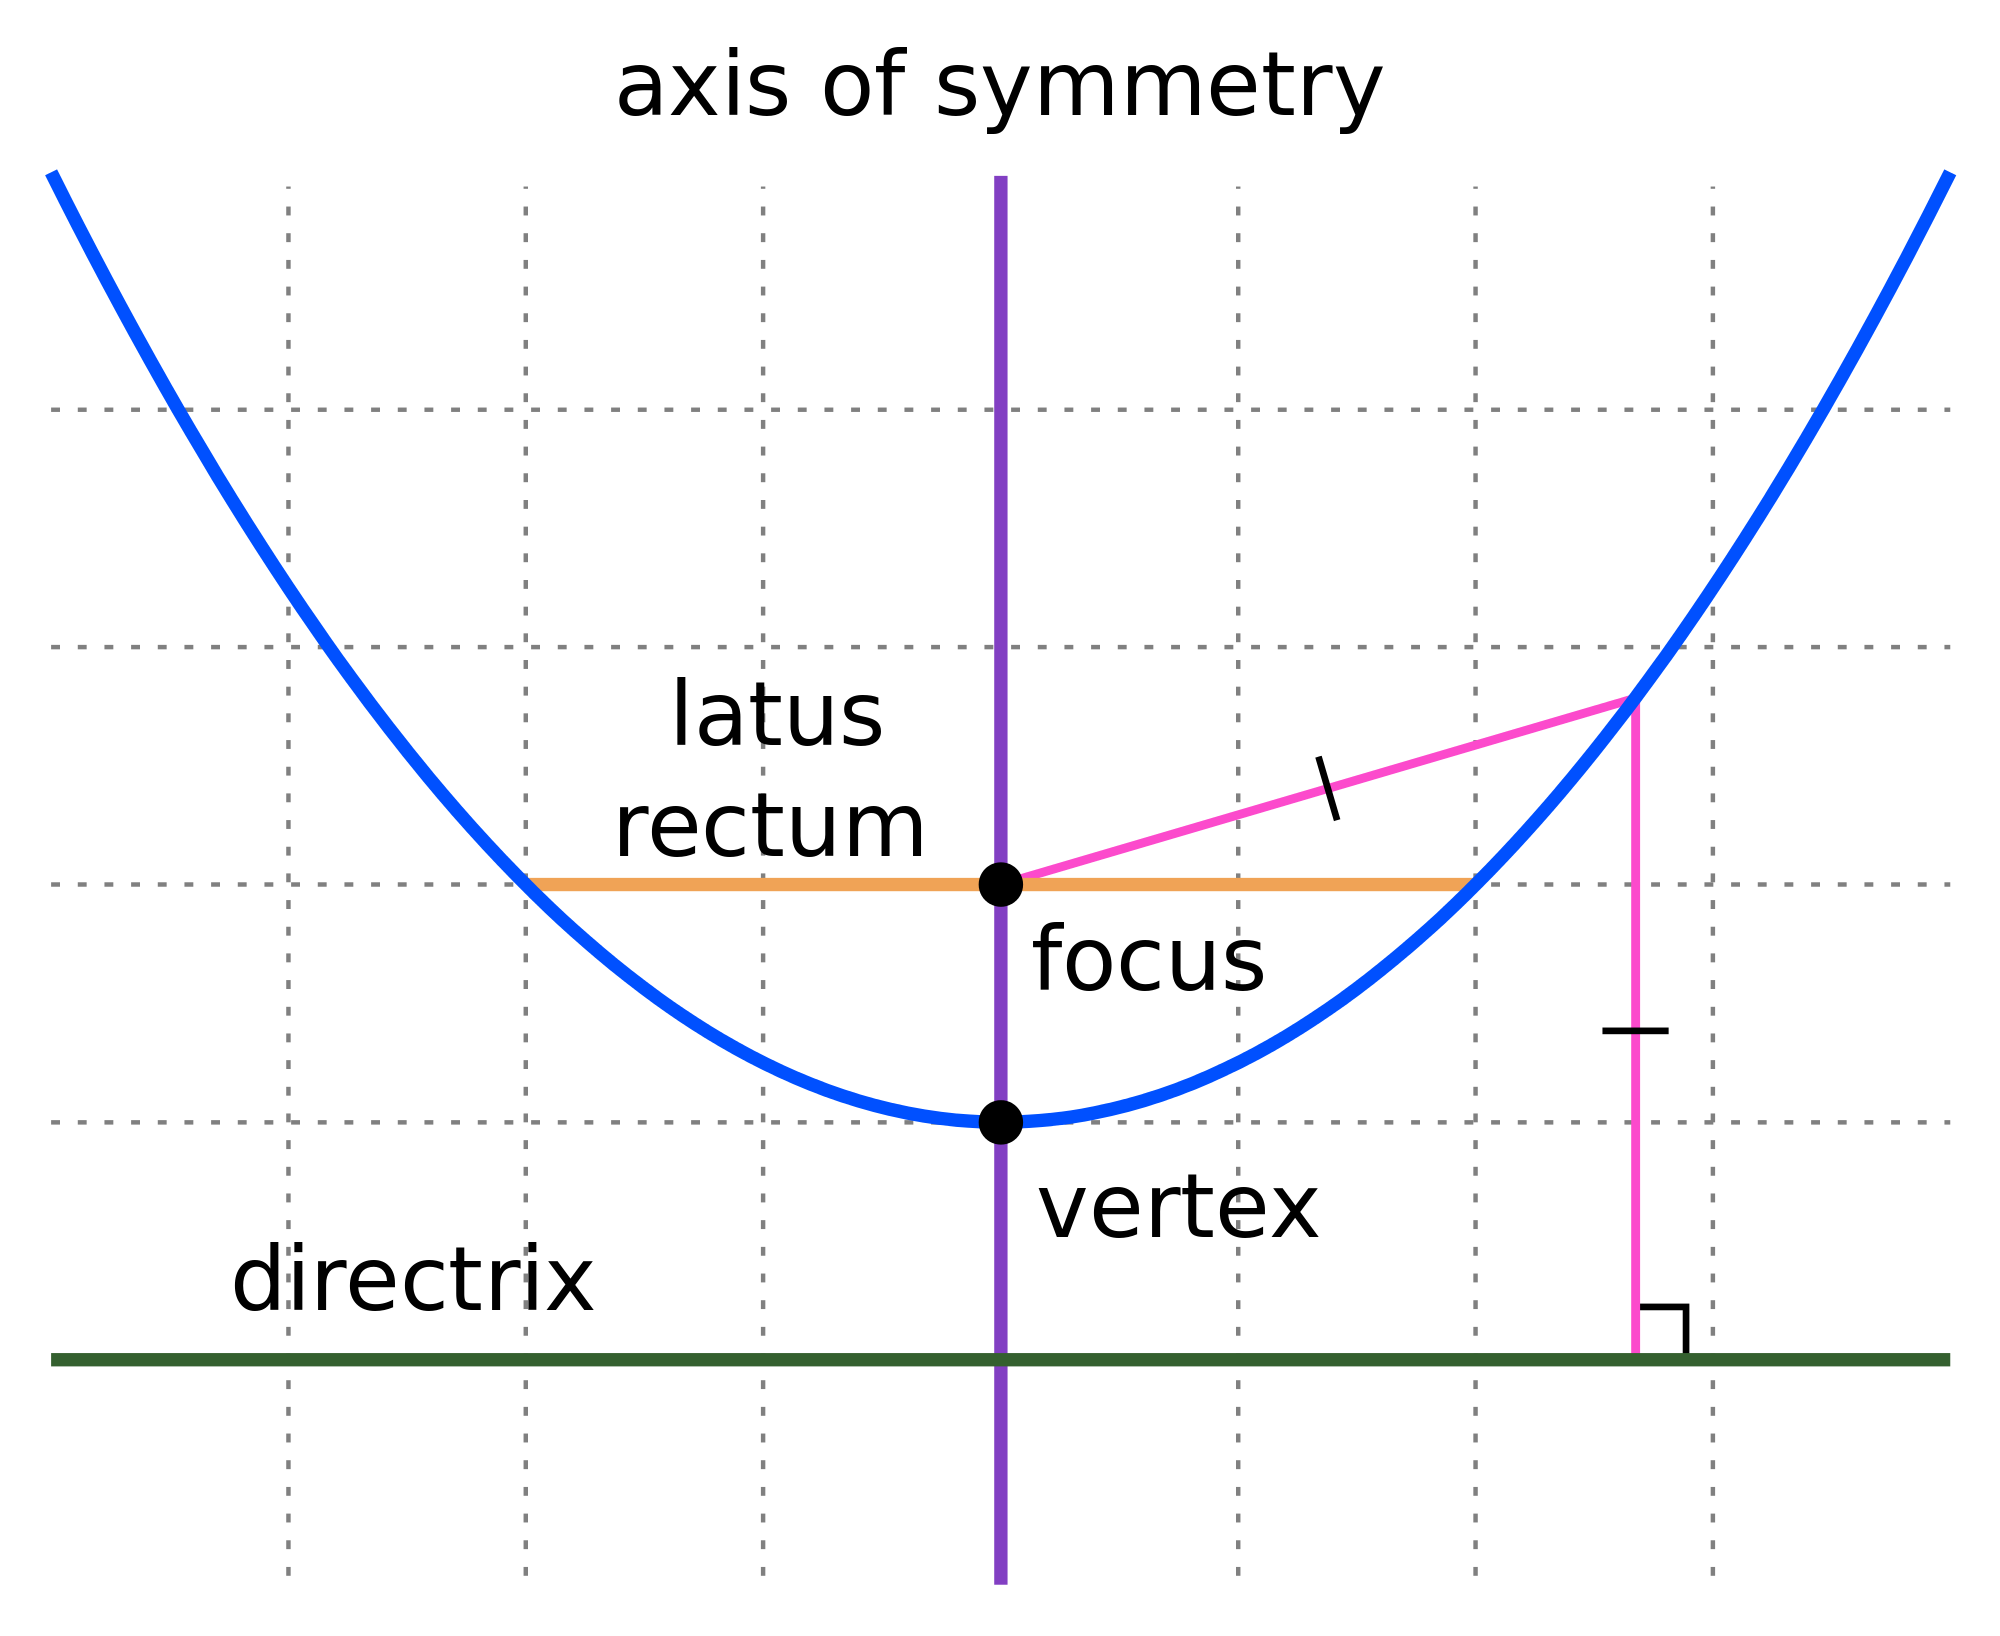
\includegraphics[width=1\textwidth,right]{parabola}
			%\centering
		\end{subfigure}
		\begin{subfigure}{0.2\textwidth}
			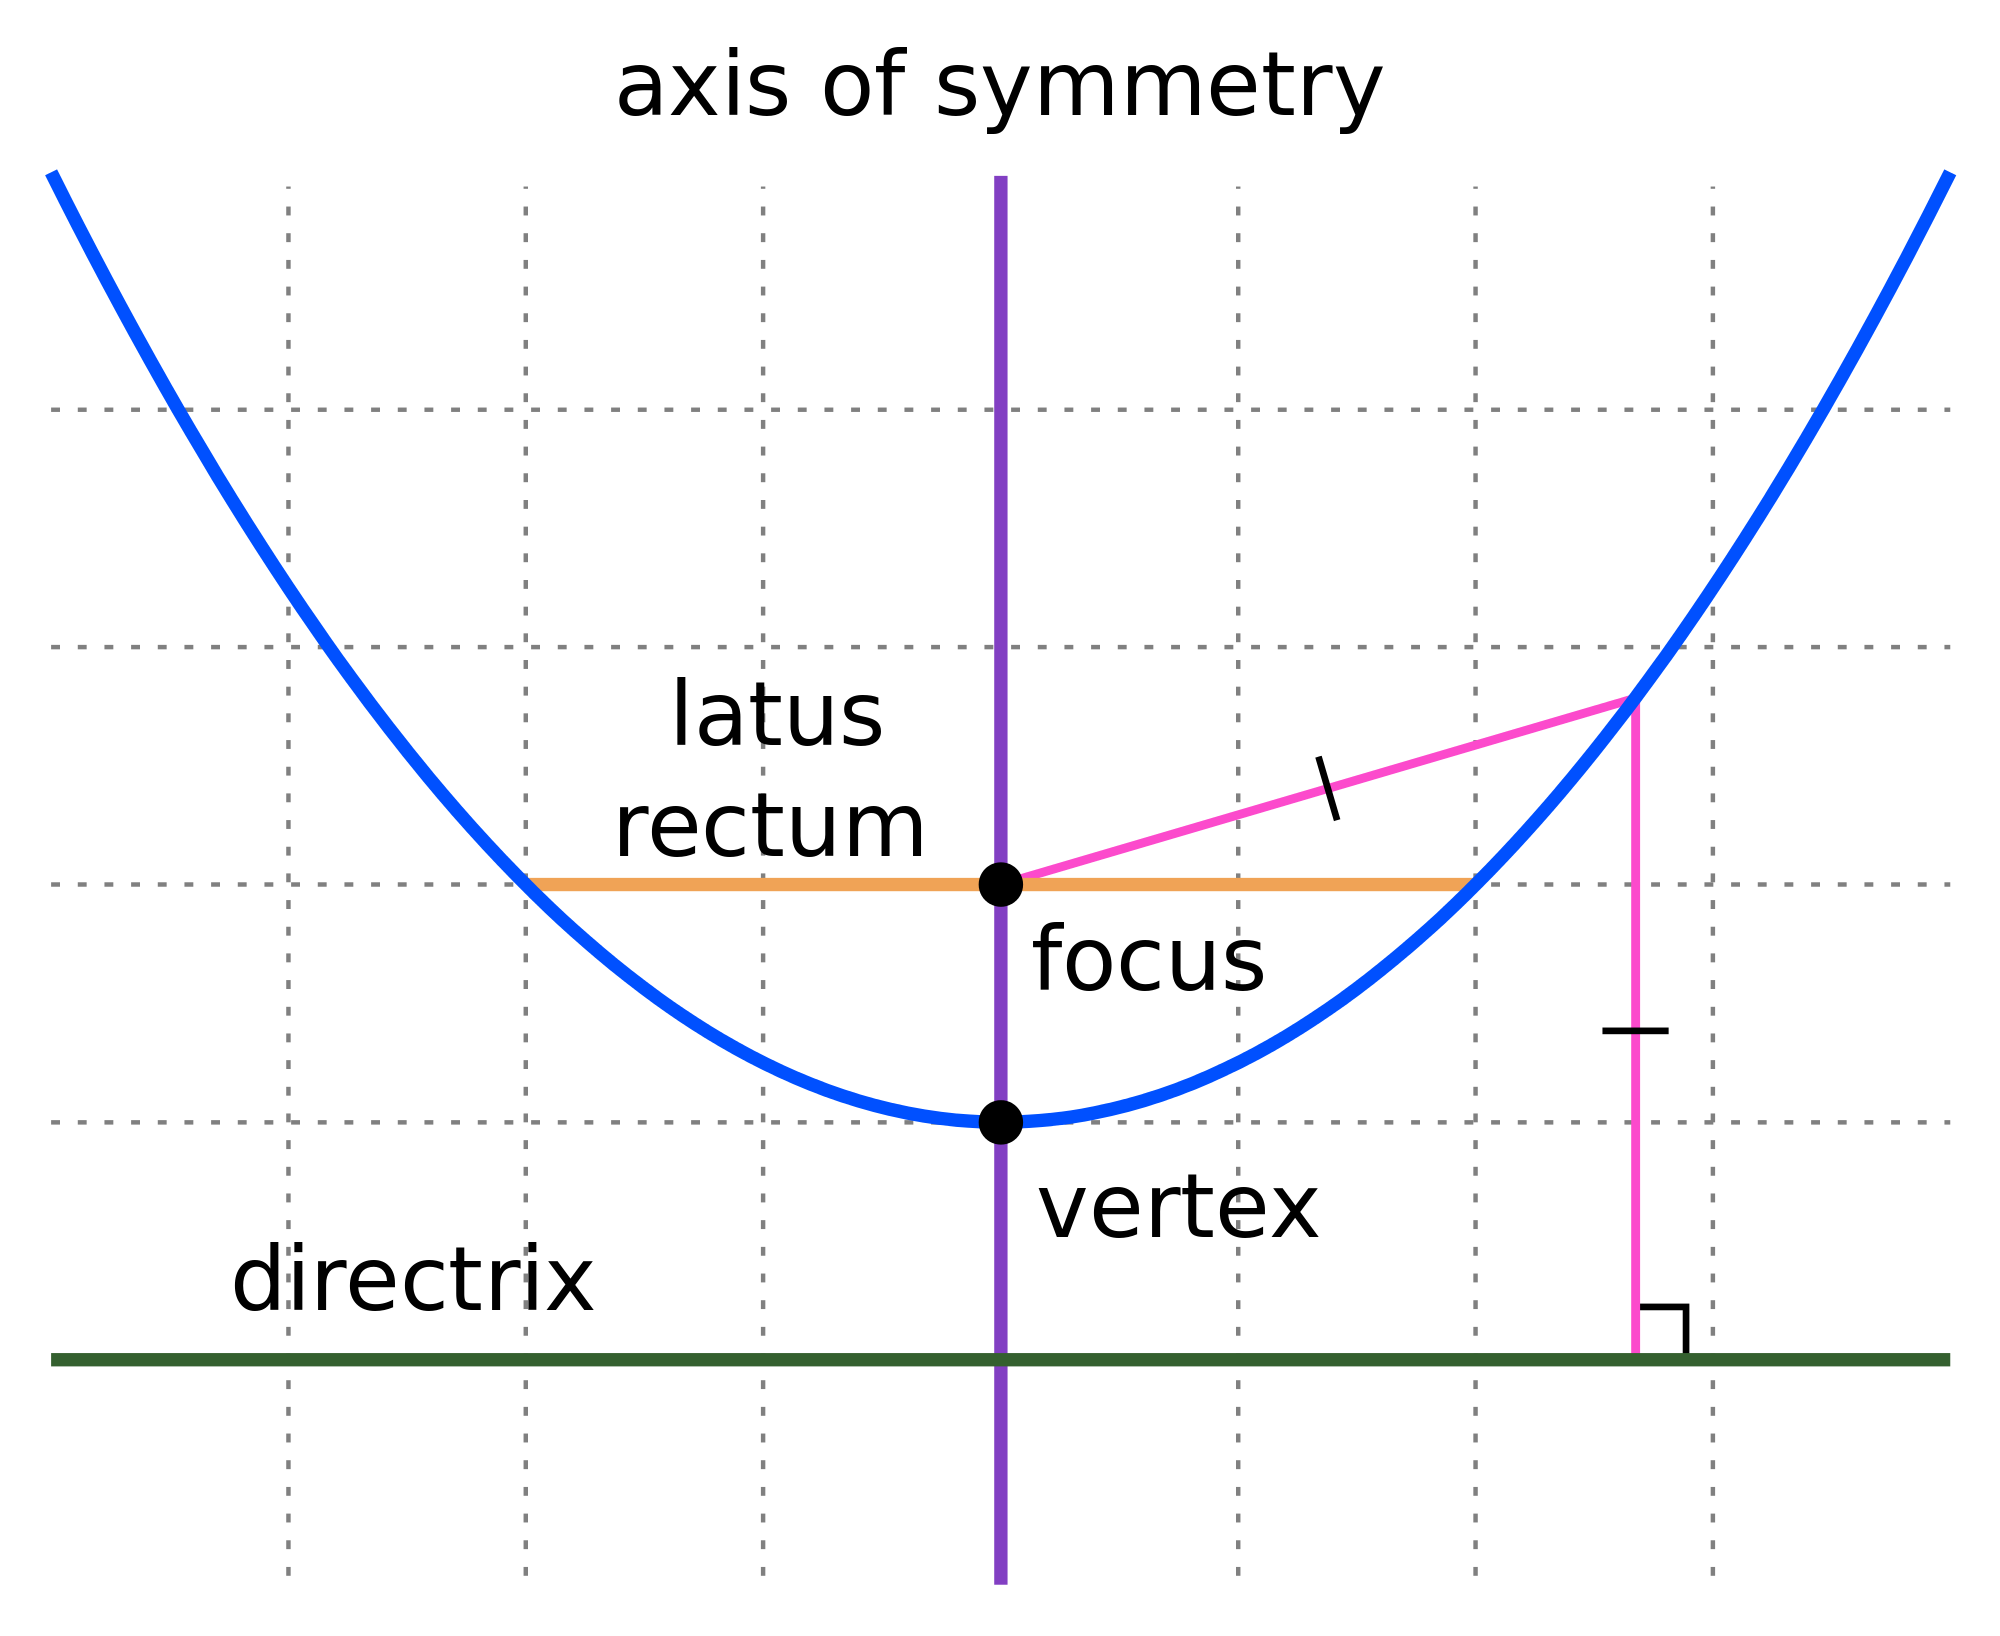
\includegraphics[width=1\textwidth,left]{parabola}
			%\centering
		\end{subfigure}
		\caption{Parabola}
	\end{figure}
	\blindtext[3]
	\lipsum
\end{document}